\chapter{Fondamentali}
L'identificazione della posizione all'interno di un edificio si svolge in 2 fasi:
\begin{enumerate}
	\item Scansione dell'ambiente
	\item Ricerca della posizione
\end{enumerate}

\section{Scansione dell'ambiente}
La scansione dell'ambiente consiste in un'analisi dell'ambiente per mezzo del magnetometro con lo scopo di registrare tutte le distorsioni del campo magnetico presenti in modo da permettere la ricerca della posizione.

\newpage
\section{Raccoglimento dei dati}
Il raccoglimento dei dati avviene tramite il magnetometro del nostro \textit{smartphone} da cui viene catturato diverse volte in un secondo il campo magnetico intorno ad esso.
Ad ogni onda magnetica viene assegnata una \textit{label}: un numero che identifica univocamente una parte dell'ambiente chiuso il cui uso verra' definito durante la fase di costruzione del modello.

\section{Onde Magnetiche}
Le onde magnetiche sono un vettore di 3 elementi, quindi in $R^3$ che classifica. Il primo valore rappresenta la forza del campo magnetico lungo l'asse X, il secondo lungo Y ed il terzo lungo Z.


\begin{figure}[H]
	\centering
	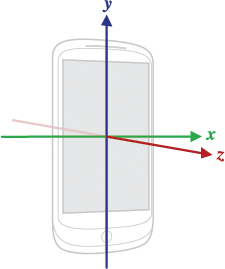
\includegraphics[width=0.20\linewidth]{./img/axis_magnetic_field.png}
	\caption{Assi x, y, z centrati sul cellulare}
	\label{fig:axis_magnetic_field}
\end{figure}


I tre valori sono espressi in $ \mu T $ (micro Tesla), unita' di misura della densita' di un flusso magnetico.
Le onde magnetiche raccolte sono dati continui sia positivi che negativi. L'intensita' dell'onda deriva dalla distorsione del campo magnetico generata dagli oggetti statici intorno al punto e dipende anche dalla velocita' con cui ci muoviamo per cui, per semplicita', assumeremo d'ora in poi una velocita' costante di 3 piedi al secondo.

\begin{figure}[H]
	\centering
	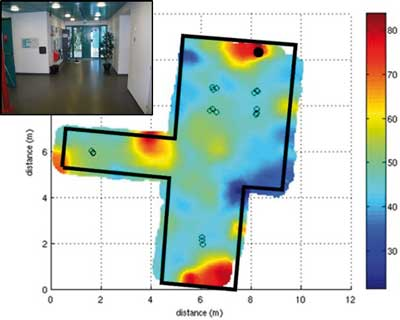
\includegraphics[width=0.7\linewidth]{img/magnetic_field_map}
	\caption[Un esempio di mappa del campo magnetico]{Mappa del campo magnetico all'universita' di Oulu: Discus Entrance hall}
	\label{fig:magneticfieldmap}
\end{figure}

\section{Elaborazione dei dati}
\subsection{Estrazione del magnitudo}
Per estrarre l'intensit\`{a} di ogni onda magnetica eseguiamo semplicemente la norma euclidea di un vettore:\\
\begin{center}
	$ \sqrt{x^2 + y^2 + z^2}$
\end{center}

\subsection{Raggruppamento}
Le onde magnetiche con la stessa \textit{label} vengono raggruppate in \textit{fingerprints}, insiemi di dimensione prefissata. A livello logico, ogni \textit{fingerprint} cerca di identificare univocamente un punto all'interno di una zona, identificata con una \textit{label}. L'insieme di \textit{fingerprints} quindi, cerca di distinguere, tramite le caratteristiche dei campi elettromagnetici di ciascun punto, ogni \textit{label} dall'altra.

\subsection{Estrazione degli attributi}
Per ogni \textit{fingerprint}, l'estrazione delle \textit{features} consiste nell'estrazione di variabili statistiche. In questo specifico caso sono:
\begin{itemize}
	\item Media
	\item Varianza
	\item Deviazione standard
	\item Mediana
	\item Media troncata
	\item Coefficiente di variazione
	\item Massimo
	\item Minimo
	\item $ 1^{\circ}, 5^{\circ}, 95^{\circ}, 99^{\circ} $ percentile
	\item $ 1^{\circ}, 2^{\circ}, 3^{\circ} $ quartile
\end{itemize}





\section{Costruzione di un modello}

Dopo aver raccolto ed elaborato le onde magnetiche, un algoritmo creera' un classificatore in grado di assegnare un'etichetta ai nuovi input ricevuti durante l'uso dell'utente finale.
Sono stati utilizzati vari classificatori per cercare il piu' preciso fra tutti. Qui di seguito introdurremo la teoria dietro ad ogni classificatore utilizzato.
\newpage
\section{IA ed Apprendimento}
La definizione secondo wikipedia\footnote{\url{https://it.wikipedia.org/wiki/Intelligenza_artificiale}} di IA e' la seguente:\\

Definizioni specifiche possono essere date focalizzandosi o sui processi interni di ragionamento o sul comportamento esterno del sistema intelligente ed utilizzando come misura di efficacia o la somiglianza con il comportamento umano o con un comportamento ideale, detto razionale:
\begin{itemize}
	\item Agire umanamente: il risultato dell'operazione compiuta dal sistema intelligente non e' distinguibile da quella svolta da un umano.
	\item Pensare umanamente: il processo che porta il sistema intelligente a risolvere un problema ricalca quello umano. Questo approccio è associato alle scienze cognitive.
	\item Pensare razionalmente: il processo che porta il sistema intelligente a risolvere un problema è un procedimento formale che si rifà alla logica.
	\item Agire razionalmente: il processo che porta il sistema
\end{itemize} 
L'apprendimento automatico e' una branca dell'intelligenza artificiale che permette al computer di apprendere da insiemi di dati per generare conoscenza con lo scopo di effettuare previsioni.

\section{Tipi di apprendimento}
Esistono 3 tipi di apprendimento:
\begin{itemize}
	\item Apprendimento supervisionato: al calcolatore vengono forniti esempi del tipo (\textbf{x}, y) per poter apprendere. L'obbiettivo della predizione per nuovi input sara' quello di calcolare la variabile dipendente. Y puo' essere sia dicreta che continua: nel primo caso si parla di classificazione, nel secondo di regressione.
	
	
	\begin{figure}[H]
		\centering
		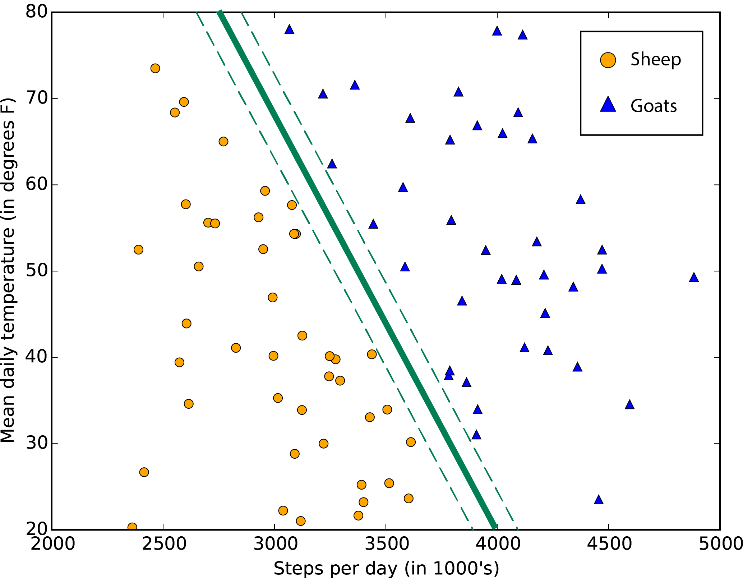
\includegraphics[width=0.7\linewidth]{img/supervised_learning_example}
		\caption{Un esempio grafico di insieme d'addestramento ed una sua classificazione}
		\label{fig:supervisedlearningexample}
	\end{figure}
	
	
	\begin{figure}[H]
		\centering
		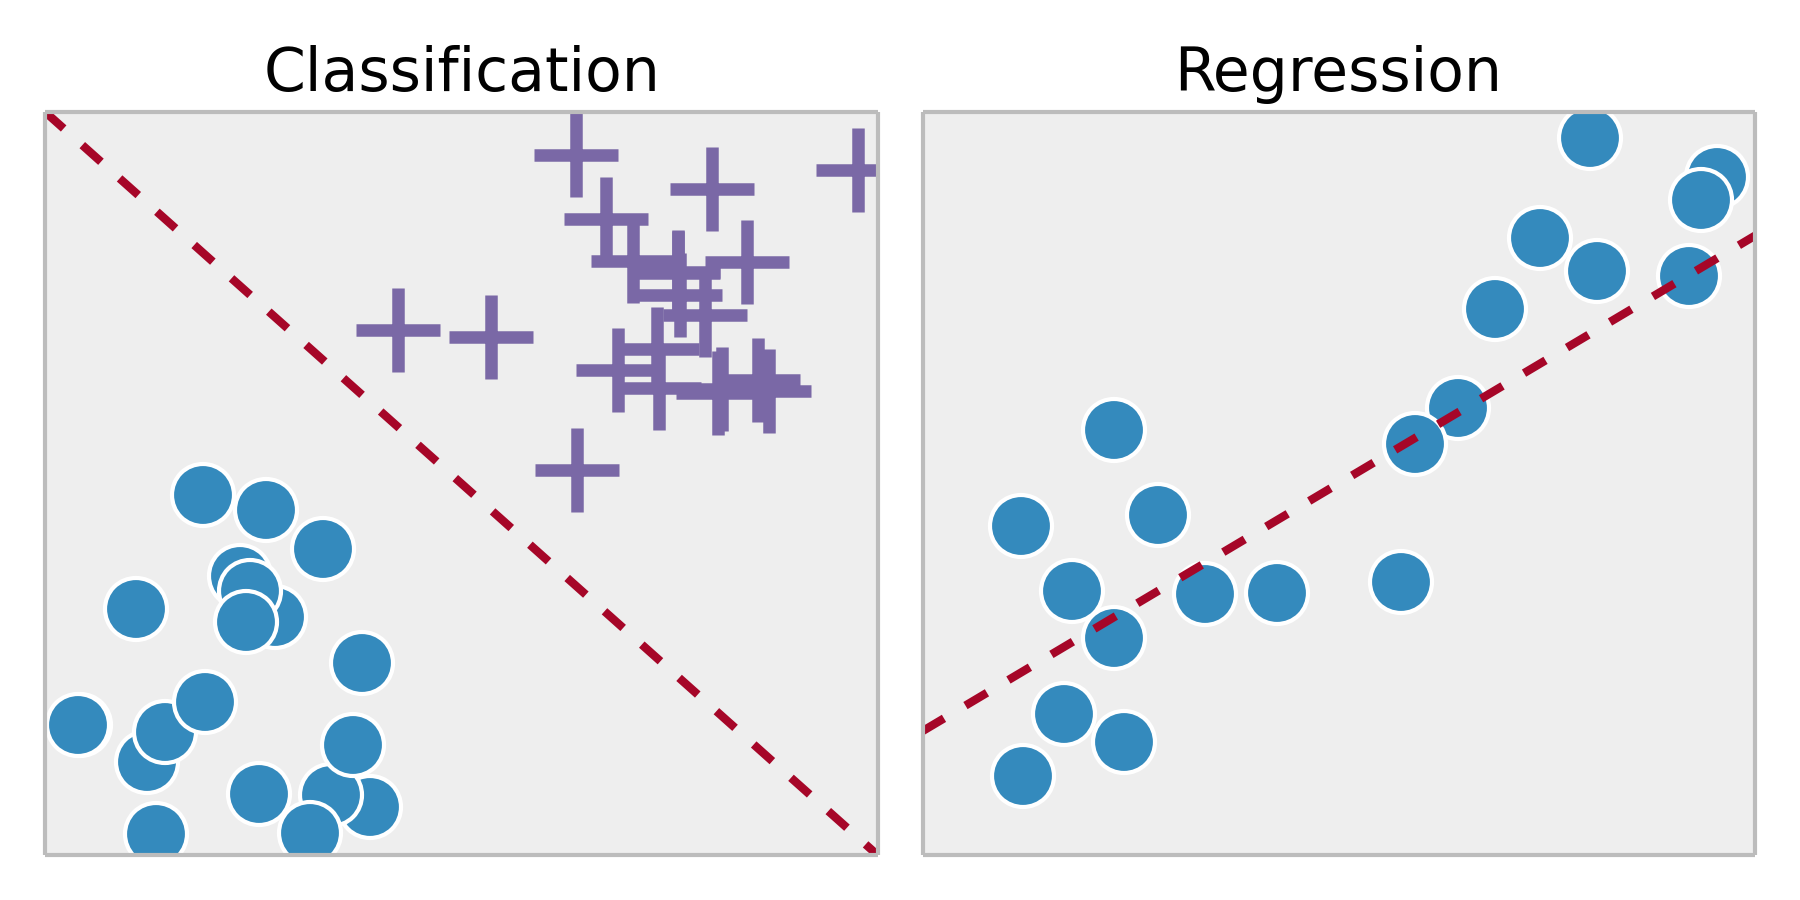
\includegraphics[width=0.7\linewidth]{img/Classification_Regression}
		\caption{Classificazione e regressione a confronto}
		\label{fig:classificationregression}
	\end{figure}

	\item Apprendimento non supervisionato: Gli esempi non contengono una variabile dipendente ma solo un insieme di attributi \textbf{x}. L'obbietto e' quello di inferire pattern nascosti dai dati non etichettati. Un'importante applicazione e' il \textit{clustering}: raggruppare i dati in base ad una similarita' fra di essi.
	
	\begin{figure}[H]
		\centering
		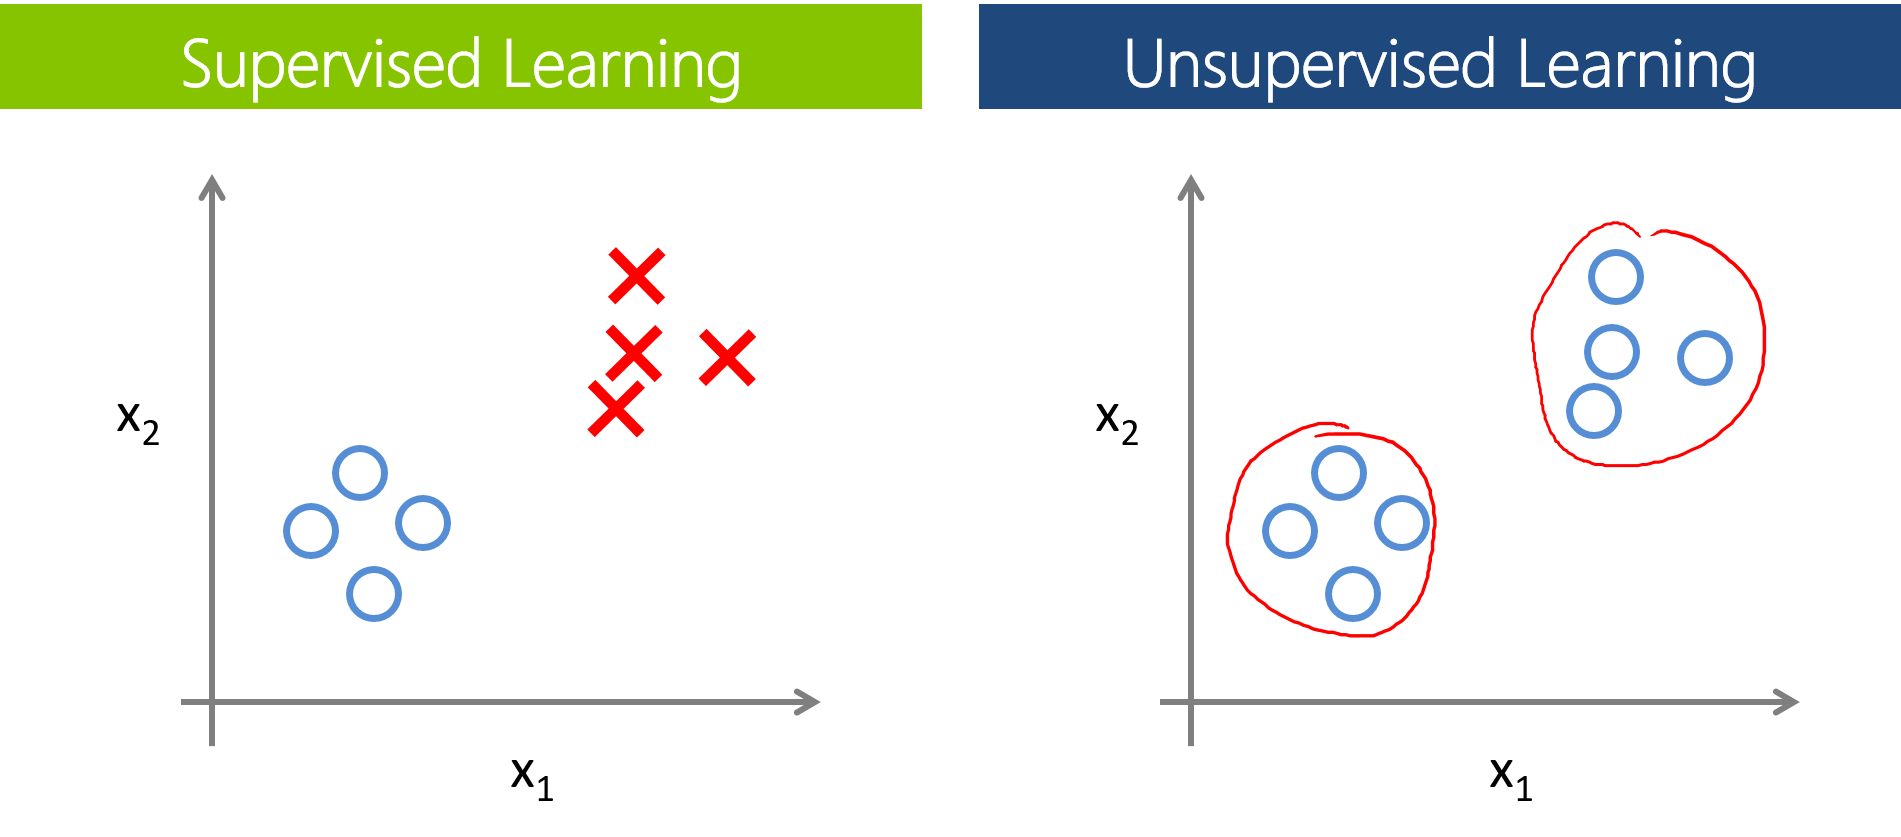
\includegraphics[width=0.7\linewidth]{img/supervised_and_unsupervised_learning}
		\caption{Apprendimento supervisiono e non supervisionato a confronto}
		\label{fig:supervisedandunsupervisedlearning}
	\end{figure}
	
	
	\item Apprendimento con rinforzo: per apprendere viene fornita una funzione ricompensa cioe' una funzione che, data un'azione effettuata dall'agente, restituira' una ricompensa di tipo numerico.
	
	\begin{figure}[H]
		\centering
		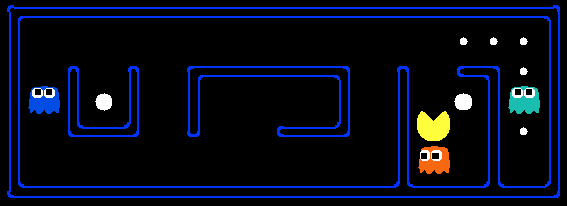
\includegraphics[width=0.7\linewidth]{img/pacman}
		\caption{L'apprendimento con rinforzo e' molto adatto ai giochi, come per esempio pacman}
		\label{fig:pacman}
	\end{figure}
	
	
\end{itemize}


\section{Alcune nozioni sull'apprendimento automatico}
\subsection{Verifica delle prestazioni}
Per verificare la correttezza del classificatore viene diviso in 2 parti il \textit{dataset} a nostra disposizione: il primo si chiama insieme di addestramento mentre il secondo insieme di test. Il nostro classificatore si allenera' sull'insieme di addestramento, cioe' imparera' dagli esempi come classificare i nuovi input ed effetuera' le predizioni sull'insieme di test, su cui verranno misurate le prestazioni in base al rapporto fra predizioni corrette e totali.

\subsection{Rumore e sovradattamento}
Un problema molto comune durante l'addestramento dei classificatori e' il rumore: durante la discriminazione degli esempi, ci ritroviamo ad un punto in cui gli attributi rimanenti sono identici ma con etichetta differente. Una probabile causa potrebbe essere la presenza di errori nei dati mentre una possibile soluzione consisterebbe nel voto di maggioranza.
Un'altro problema e' il sovradattamento: la costruzione di un classificatore consistente con tutti gli esempi a causa dell'utilizzo di attributi irrilevanti nella classificazione. Supponiamo di voler predire l'esito del lancio di un dado e fra gli attributi di avere ora, giorno, mese ed anno; ecco un esempio lampante di sovradattemento. Nei casi reali tuttavia non sono cosi' evidenti gli attributi insignificanti e, per esempio, una tecnica utilizzata  negli alberi di decisione e' la potatura.

\begin{figure}[H]
	\centering
	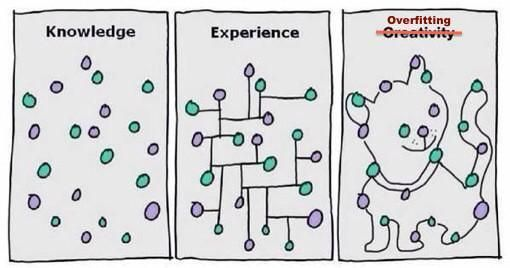
\includegraphics[width=0.7\linewidth]{img/overfitting}
	\caption{}
	\label{fig:overfitting}
\end{figure}


\subsection{Cross validation}
Per migliorare le performance di un classificatore si suddivide l'intero \textit{dataset} in $n$ parti uguali (di solito 10), ognuna delle quali svolgera' per una volta il ruolo di insieme di test mentre il resto sara' l'insieme di addestramento. Questa tecnica risolve vari problemi tra i quali l'\textit{overfitting}.\\

\begin{figure}[H]
	\centering
	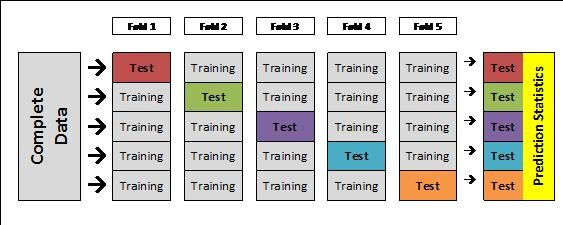
\includegraphics[width=0.7\linewidth]{img/crossvalidation}
	\caption{Rappresentazione grafica della Cross Validation}
	\label{fig:crossvalidation}
\end{figure}


\section{K Nearest Neightbour}
Uno degli algoritmi piu' semplici di apprendimento automatico, e' il \textit{k-nearest-neightbours} dove l'input consiste in $k$ elementi presi dal \textit{training set} piu' vicini in base ad un criterio scelto da chi utilizza l'algoritmo (per esempio la distanza euclidea o di Mahalanobis). Il KNN viene definito un algoritmo pigro(\textit{lazy}) perche' non ha bisogno di apprendere dall'insieme di addestramento per poter creare un classificatore ma puo' usare direttamente i dati forniti per classificare i nuovi esempi. L'inconveniente che abbiamo ricade sul costo computazione: esso e' proporziale alla grandezza del dataset.


\begin{figure}[H]
	\centering
	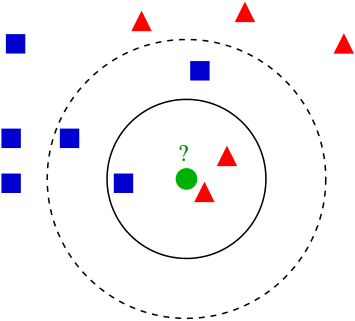
\includegraphics[width=0.7\linewidth]{img/knn_example}
	\caption{Esempio grafico dell'algoritmo KNN}
	\label{fig:knnexample}
\end{figure}


\subsection{Scelta del parametro k}
La scelta del parametro dipende, ovviamente, dal tipo dei dati che abbiamo e dalla quantita', anche se in generale piu' e' grande $k$ meno rumore viene generato da questo algoritmo. Un buon metodo per trovare il giusto valore e' l'uso di tecniche euristiche, come la \textit{cross validation}. Un altra fonte di rumore di cui bisogna stare attenti e' la presenza di \textit{features} insignificanti nella ricerca del vicino. Per porre rimedio possiamo, ad esempio, usare un algoritmo genetico per selezionare le \textit{features} piu' significative

\section{Naive bayes}
Un altro tipo di apprendimento usato per classificare le \textit{label} e' Naive bayes: un algoritmo di classificazione e regressione basato sulla statistica. Prima di spiegare in cosa consiste occorre spiegare un paio di concetti:
\subsection{Teorema di bayes}
Il teorema di bayes ci fornisce una relazione fra probabilita' condizionate molto utile nel calcolo probabilistico ma anche per l'apprendimento automatico. L'equazione e' la seguente:
\begin{center}
	$P(B|A) = \dfrac{P(A|B)P(B)}{P(A)}$
\end{center}
\subsection{Rete bayesiana}
Una rete bayesiana e' un grafo diretto aciclico i cui nodi sono le variabili casuali del sistema mentre gli archi rappresentato la condizione di dipendenza fra nodi.
 Ad ogni nodo e' associata una tabella di distribuzione delle probabilita' la cui complessita' e' proporzionale al numero di archi entranti.\\ Per esempio se il nodo con variabile casuale Leggere ha un arco verso Istruito allora possiamo dire che Istruito e' condizionalmente dipendente da Leggere. Qui sotto potete vedere una raffigurazione grafica di una semplice rete bayesiana formata da nodi padre ed un figlio:
\begin{figure}[H]
	\centering
	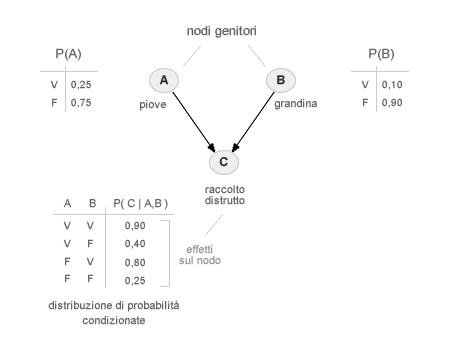
\includegraphics[width=0.7\linewidth]{img/rete-bayesiana-grafo.png}
	\caption{Esempio di rete bayesiana}
	\label{fig:rete-bayesiana-grafo}
\end{figure}
\medskip
\subsection{Naive Bayes}
Naive bayes e' una rete bayesiana in cui si assume l'indipendenza condizionale fra tutte le variabili casuali del sistema data la classe. Questa forte assunzione non mira a modellare esattamente la realta' ma fornisce delle buone performance sulla predizione di una classe.

\begin{figure}[H]
	\centering
	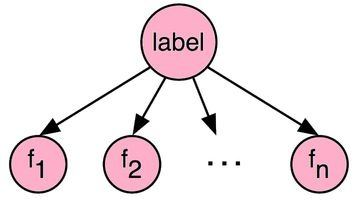
\includegraphics[width=0.4\linewidth]{img/naive_bayes_example}
	\caption{Esempio di rete bayesiana ingenua}
	\label{fig:naivebayesexample}
\end{figure}

\subsection{Costruzione di una rete bayesiana ingenua}
Preso l'insieme di esempi, ricavare la tabella di distribuzione delle probabilita' al variare di tutti i valori che la variabile dipendente puo' assumere. Successivamente costruire un grafo che ha come nodo radice la variabile dipendente e come figli tutte le variabili indipendenti.
\medskip
\subsection{Predizione di risultati}
Preso un insieme di attributi $\textbf{x}$ con valori $x_1x_2x_3...x_n$ e tutti i valori della variabile dipendente $\textbf{y}=y_1y_2y_3...y_m$ , per classificare l'insieme applicheremo il teorema di bayes con un'approssimazione molto usata nel campo scientifico chiamata MAP (Massima ipotesi a posteriori)
\begin{align*}
		etichetta &=y_j \, in \, \max_j\,P(y_j|X_1=x_1, X_2=x_2...X_N=x_n) \\
		&= \max_j \dfrac{P(X_1=x_1,X_2=x_2...X_N=x_n|y_j)P(y_j)}{P(X_1=x_1, X_2=x_2...X_N=x_n)}\\
		&= \max_j \dfrac{\prod_iP(x_i|y_j)P(y_j)}{P(X_1=x_1, X_2=x_2...X_N=x_n)}
\end{align*}

i cui valori della precedente equazione si possono ricavare dalla tabella di distribuzione delle probabilita'.

\subsection{Modelli generativi e discriminativi}
L'espressione $P(y_j|\textbf{x})$ puo' essere calcolata in modi differenti in base al modello trattato: nel caso di modelli discriminativi, l'espressione viene ricavata direttamente dai dati sorgente mentre nei modelli generativi l'obbiettivo e' di costruire una distribuzione congiunta di probabilita' per $P(\textbf{x}, y_j)$ oppure da $P(\textbf{x}| y_j)$ e $P(y_j)$.

\subsection{Calcolo della probabilita' a priori}
  Per calcolare la probabilita' a priori esistono varie tecniche: l'equiprobabilita' $\left(\dfrac{1}{|\textbf{y}|}\right)$, rapporto fra esempi di classe $j$ e il totale degli esempi dall'insieme di addestramento, le distribuzioni di probabilita' oppure un modello non parametrico dall'insieme di addestramento.
  
\subsection{Modelli ad eventi}  
   La distribuzione viene anche chiamata modello ad eventi perche' tratta gli attributi come probabilita' di eventi. Ci sono 3 modelli usati con $\textit{Naive Bayes}$ che sono:
\begin{itemize}
	\item Bernoulli: gli attributi sono di tipo \textit{booleano} e l'attributo $x_i \in \textbf{x}=(x_1,x_2,...,x_n)$ vale 1 se l'evento $i$ e' avvenuto, 0 altrimenti. Nel caso bernoulliano possiamo valutare $P(\textbf{x}|y_j)$ come
	\begin{center}
	 $P(\textbf{x}|y_j) = \prod_{j=1}^{n} P_{ij}^{x_i} (1-P_{ij})^{(1-x_i)}$
	\end{center}
	Dove $P_{ij}$ e' la probabilita' per $y_j$ che $x_i$ sia vero. Un esempio canonico e' quello della classificazione dei documenti, dove $x_i$ rappresenta la presenza del termine $w_j$ nei documenti di classe $y_j$ e di conseguenza $P_{ij}$ la probabilita' di trovarlo. Dobbiamo notar bene che Bernoulli a differenza della multinomiale valuta nella produttoria anche la probabilita' che l'evento $i$ non avvenga.
	

	\item Multinomiale: Nella multinomiale gli esempi rappresentano la frequenza con il quale gli eventi sono stati generati dalla multinomiale $(p_1...p_n)$ dove $p_i$ e' la probabilita' che $i$ occorra. Gli attributi $\textbf{x}=(x_1,x_2...x_n)$ contano quante volte l'evento $i$ e' avvenuto. La probabilita' condizionata  $P(\textbf{x}|y_j)$ e' stimata come
	\begin{center}
		$P(\textbf{x}|y_i) = \dfrac{(\sum_{i}x_i)!}{\prod_{i}x_i!}\prod_i p_{ki}^{x_i}$
	\end{center}
	\item Gaussiana: viene utilizzata con dati continui e si assume che siano distribuiti in base alla Gaussiana. Per ogni classe $y_j$, viene ricavata la media $\mu_j$ e la varianza $\sigma_{j}^{2}$. Supponiamo di aver raccolto un insieme di valori $v$ allora la probabilita' sara':
	\begin{center}
		$P(x =v | y_j) = \dfrac{1}{\sqrt{2 \pi \sigma_{j}^2}} e^{-\dfrac{(v - \mu_j)^2}{2 \sigma_{j}^2}}$
	\end{center}
	Un'altra possibile opzione per trattare valori continui e' la discretizzazione da cui possiamo utilizzare Bernoulli/Multinomiale anche se bisogna stare attenti a non perdere informazioni discriminanti.
\end{itemize}

\subsection{Un piccolo esempio basato su naive bayes}
Supponiamo di dover usare Naive Bayes per predire se giocare una partita di tennis o no in base alle condizioni meteorologiche. Dati gli esempi qui sotto a sinistra, possiamo ricavare la tabella di distribuzione delle probabilita' generale come qui di seguito:
\begin{figure}[H]
	\centering
	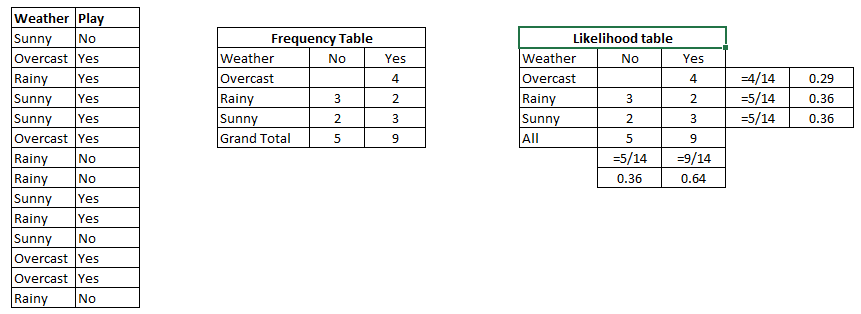
\includegraphics[width=1\linewidth]{img/Bayes_tennis_sample}
	\caption{Esempi di partite di tennis giocate in base alle condizioni meteorologiche e tabella di distribuzione delle probabilita'}
	\label{}
\end{figure}
\medskip
Ecco una rappresentazione grafica di \textit{Naive Bayes}:\\\\

\begin{figure}[H]
	\centering
	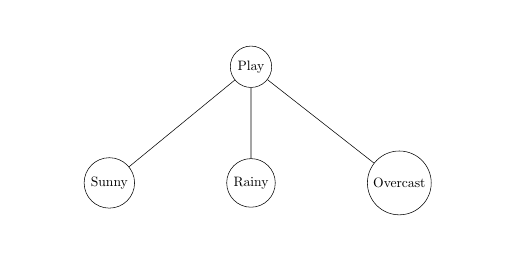
\includegraphics[width=0.7\linewidth]{img/graph_naive_bayes}
	\caption{}
	\label{fig:graphnaivebayes}
\end{figure}

%	\begin{tikzpicture} 
%		\node[draw, circle](0){Play}
%		child{ node(1)[draw, circle, left]{Sunny}}
%		child{	 	node(2)[draw, circle]{Rainy}}
%		child{	  node(3)[draw, circle, right]{Overcast} };
%	\end{tikzpicture}
\section{Alberi di decisione}
Gli alberi di decisione sono un altro tipo di apprendimento supervisionato, quindi dovremmo avere 
Da un punto di vista strutturale, l'albero di decisione e' un albero (inteso come struttura dati) dove i nodi interni sono gli attributi, i rami tutti i possibili valori assumibili dall'attributo (oppure un range nel caso continuo) e le foglie sono la predizione da scegliere\\D'ora in poi parleremo, per semplicita', solo di classificazione quando non espresso chiaramente.

\subsection{Costruzione di un albero di decisione}
L'albero di decisione si potrebbe definire prendendo a caso un attributo ed iniziare a dividere gli esempi fino ad ottenere foglie, anche se cosi' otterremo un albero  non molto utile in tutti i casi in cui non abbiamo gli esempi. Quindi quale albero scegliere fra tutti quelli possibili? In questo caso ci aiuta il rasoio di Occam, che ci dice di scegliere quello piu' piccolo fra tutti. Per generare l'albero piu' piccolo dovremmo scegliere gli attributi piu' significativi per generare l'albero. Cosa intendiamo per significativo? Intendiamo l'attributo che genera figli con meno varieta' di classi presenti all'interno di essi.\\ Un esempio: immaginiamo di avere 10 esempi con attributi A e B e come valore associato un booleano. se abbiamo l'attributo A che genera due figli con esempi aventi meta' valore vero e falso mentre se suddividiamo secondo B abbiamo figli con esempi esclusivamente veri oppure falsi. In questo caso indubbiamente l'attributo piu' significativo e' B.

\subsection{Classificazione dei nuovi elementi}
Quando dovremmo predire l'etichetta di un nuovo insieme di attributi $x$ bastera' semplicemente scorrere l'albero di decisione dalla radice fino ad una foglia, che sara' l'etichetta da assegnare.

\subsection{Un esempio di albero di decisione}
Riprendiamo l'esempio della partita di tennis, questa volta con qualche attributo in piu'. La tabella e' la seguente:
\begin{figure}[H]
	\centering
	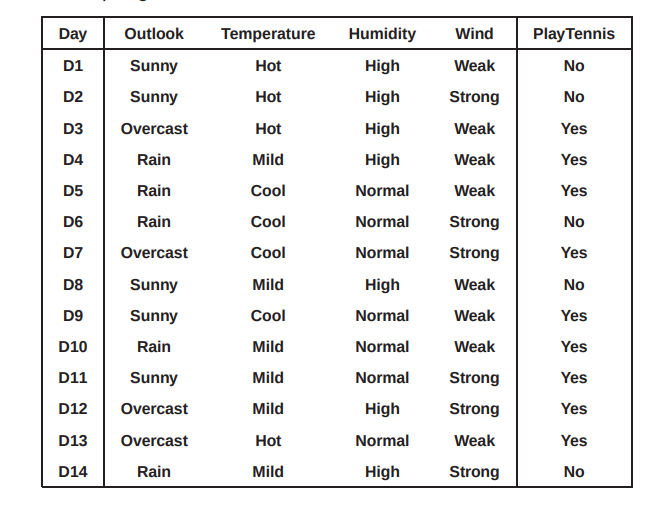
\includegraphics[width=0.7\linewidth]{img/decision-_tree_table_tennis}
	\caption{Tabella degli attributi meteorologici con valore associato un booleano che stabilisce se la partita e' stata giocata o no}
	\label{fig:decision-treetabletennis}
\end{figure}
da cui possiamo ricavare il seguente albero di decisione:
\begin{figure}[H]
	\centering
	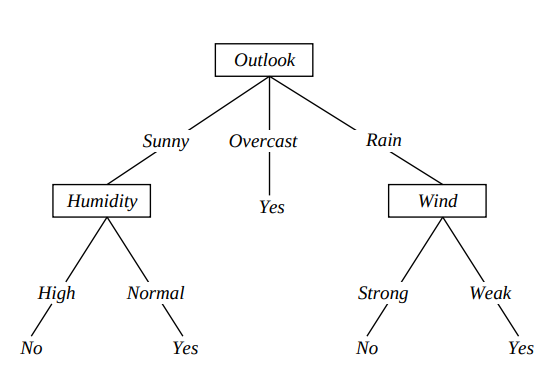
\includegraphics[width=0.7\linewidth]{img/decision_tree_tree_tennis}
	\caption{Albero di decisione ricavato dalla tabella precedente}
	\label{fig:decisiontreetreetennis}
\end{figure}

\section{Ricerca della posizione}
Dopo la costruzione del modello esso viene adoperato per predire la posizione corrente dell'utente che esegue l'applicazione. La ricerca consiste nel creare sul momento una \textit{fingerprint} e poi, tramite un algoritmo di classificazione, cercare di inferire la \textit{label}  su cui ci troviamo. Gli algoritmi utilizzati per analizzare il problema sono quelli descritti in precedenza quindi
\begin{enumerate}
	\item \textit{K Nearest Neightbour}
	\item Bayes ingenuo
	\item  Alberi di decisione
\end{enumerate}
\newpage
